\let\negmedspace\undefined
\let\negthickspace\undefined
\documentclass[journal]{IEEEtran}
\usepackage[a5paper, margin=10mm, onecolumn]{geometry}
%\usepackage{lmodern} % Ensure lmodern is loaded for pdflatex
\usepackage{tfrupee} % Include tfrupee package

\setlength{\headheight}{1cm} % Set the height of the header box
\setlength{\headsep}{0mm}     % Set the distance between the header box and the top of the text

\usepackage{gvv-book}
\usepackage{gvv}
\usepackage{cite}
\usepackage{amsmath,amssymb,amsfonts,amsthm}
\usepackage{algorithmic}
\usepackage{graphicx}
\usepackage{textcomp}
\usepackage{xcolor}
\usepackage{txfonts}
\usepackage{listings}
\usepackage{enumitem}
\usepackage{mathtools}
\usepackage{gensymb}
\usepackage{comment}
\usepackage[breaklinks=true]{hyperref}
\usepackage{tkz-euclide} 
\usepackage{listings}
% \usepackage{gvv}                                        
\def\inputGnumericTable{}                                 
\usepackage[latin1]{inputenc}                                
\usepackage{color}                                            
\usepackage{array}                                            
\usepackage{longtable}                                       
\usepackage{calc}                                             
\usepackage{multirow}                                         
\usepackage{hhline}                                           
\usepackage{ifthen}                                           
\usepackage{lscape}
\begin{document}

\bibliographystyle{IEEEtran}
\vspace{3cm}

\title{1.2.25}
\author{EE24BTECH11014 - DEEPAK
}
% \maketitle
% \newpage
% \bigskip
{\let\newpage\relax\maketitle}

\renewcommand{\thefigure}{\theenumi}
\renewcommand{\thetable}{\theenumi}
\setlength{\intextsep}{10pt} % Space between text and floats


\numberwithin{equation}{enumi}
\numberwithin{figure}{enumi}
\renewcommand{\thetable}{\theenumi}




\textbf{Question: }\\

Rain is falling vertically with a speed of $ 30 ms^{-1}$. A woman rides a bicycle with a speed of $10 ms^{-1}$ in the north to south direction. What is the direction in which she should hold her umbrella?
\\
\solution :
\begin{table}[h!]    
  \centering
  \begin{tabular}[12pt]{ |c| c| c| }
    \hline
	\textbf{Variable}  & \textbf{Description}  & \textbf{value }  \\
    \hline
	$\vec{v}_{\text{rain}}$ & velocity vector of rain in vertical downwards direction & $30 ms^{-1}$\\
    \hline 
	$\vec{v}_{\text{woman}}$ & velocity vector of women in north to south (Horizontal) direction & $10 ms^{-1}$ \\
    \hline
	$\vec{v}_{\text{relative}}$& velocity of rain with respect to woman  \\  
    \hline 
        $\theta$ & angle with vertical in which she should hold her umbrella \\
    \hline    
            
\end{tabular}
  \caption{Variables Used}
  \label{tab1.1.9.2}
\end{table}



\[
\vec{v}_{rain} = \myvec{0\\-30} \text{m/s}
\]


\[
\vec{v}_{\text{woman}} = \myvec{-10\\0} \text{m/s}
\]

velocity of rain with respect to woman :
\[
\vec{v}_{\text{relative}} = \vec{v}_{\text{rain}} - \vec{v}_{\text{woman}}
\]

\[
\vec{v}_{\text{relative}} = \myvec{0\\-30} - \myvec{-10\\0}
\]

\[
\vec{v}_{\text{relative}} = \myvec{10\\-30}
\]

So, the relative velocity of the rain with respect to the woman is:
\[
\vec{v}_{\text{relative}} = \myvec{10\\-30}, \text{m/s}
\]


The direction in which she should hold the umbrella is the direction of the relative velocity vector. \\
since $\theta$ is the angle with the vertical \\so,
\[
\tan \theta =  \frac{10}{-30} = -\frac{1}{3}
\]

Thus, the angle \( \theta \) is:
\[
\theta = \tan^{-1}(-\frac{1}{3})
\]
    \begin{figure}[h]
        \centering
       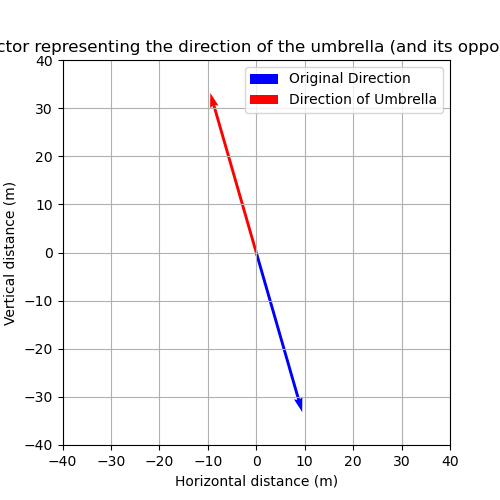
\includegraphics[width=\linewidth]{figs/fig1.png}
       \caption{}
       \label{graph}
    \end{figure}

\end{document}
